\documentclass{standalone}
\usepackage{tikz}
\usetikzlibrary{patterns, positioning}
\usepackage[sfdefault]{ClearSans} %% option 'sfdefault' activates Clear Sans as the default text font
\usepackage[T1]{fontenc}

\begin{document}
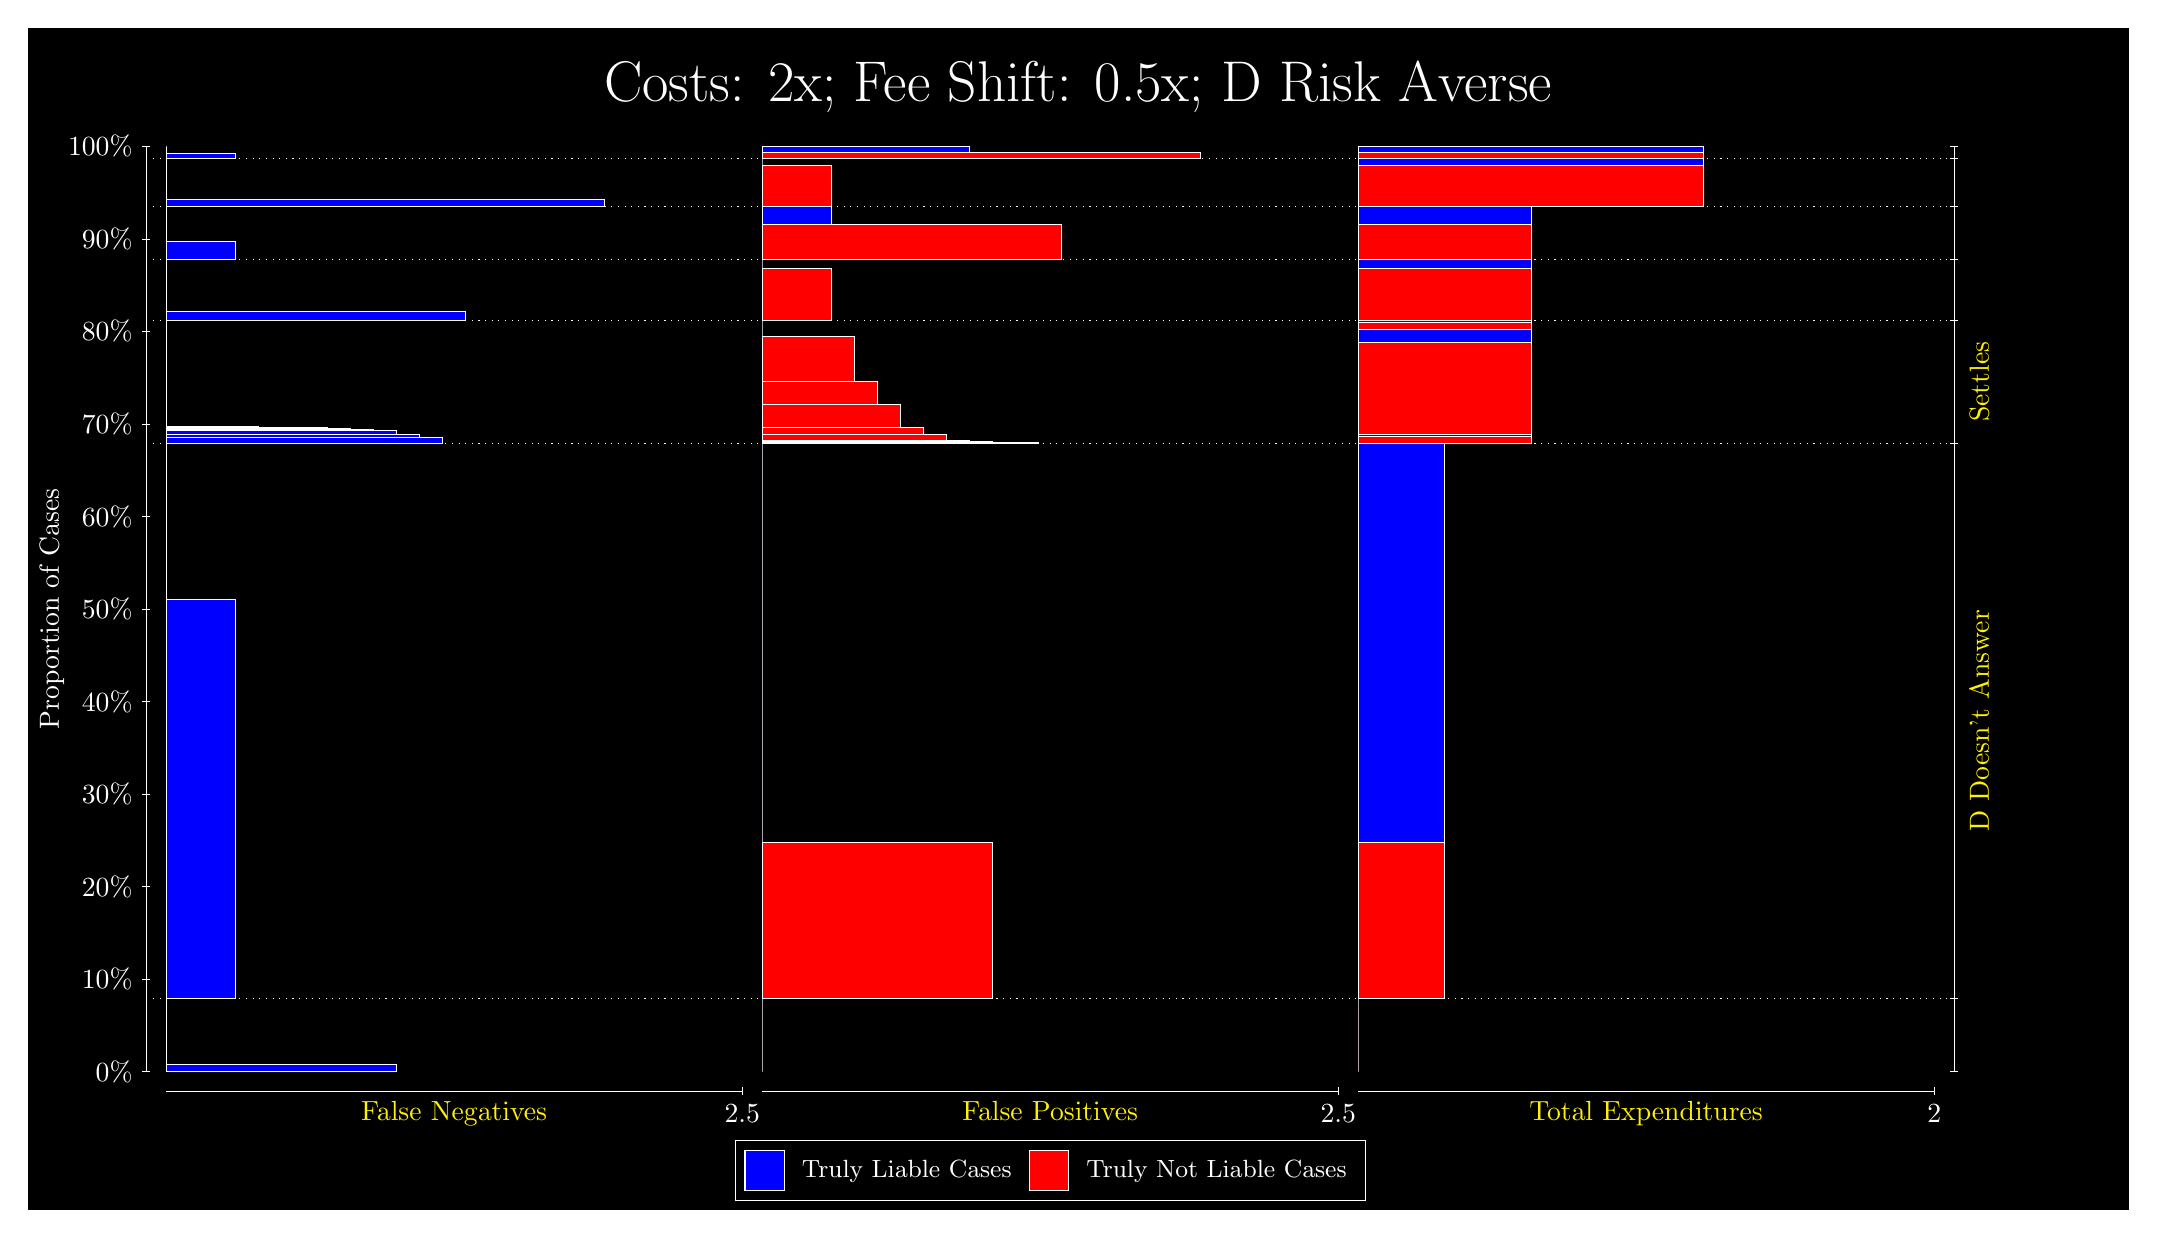
\begin{tikzpicture}
\draw[fill=black] (0,0) rectangle (26.667,15);
\draw[text=white] (0,13.5) rectangle (26.667,15) node[midway] {\huge Costs: 2x; Fee Shift: 0.5x; D Risk Averse};
\draw[white, very thin] (1.5,1.75) -- (1.5,13.5);
\node[rotate=90, text=white, anchor=center] at (0.3, 7.625) {Proportion of Cases};
\draw[white, very thin] (1.45,1.75) -- (1.55,1.75);
\node[text=white, anchor=east] at (1.45, 1.75) {0\%};
\draw[white, very thin] (1.45,2.925) -- (1.55,2.925);
\node[text=white, anchor=east] at (1.45, 2.925) {10\%};
\draw[white, very thin] (1.45,4.1) -- (1.55,4.1);
\node[text=white, anchor=east] at (1.45, 4.1) {20\%};
\draw[white, very thin] (1.45,5.275) -- (1.55,5.275);
\node[text=white, anchor=east] at (1.45, 5.275) {30\%};
\draw[white, very thin] (1.45,6.45) -- (1.55,6.45);
\node[text=white, anchor=east] at (1.45, 6.45) {40\%};
\draw[white, very thin] (1.45,7.625) -- (1.55,7.625);
\node[text=white, anchor=east] at (1.45, 7.625) {50\%};
\draw[white, very thin] (1.45,8.8) -- (1.55,8.8);
\node[text=white, anchor=east] at (1.45, 8.8) {60\%};
\draw[white, very thin] (1.45,9.975) -- (1.55,9.975);
\node[text=white, anchor=east] at (1.45, 9.975) {70\%};
\draw[white, very thin] (1.45,11.15) -- (1.55,11.15);
\node[text=white, anchor=east] at (1.45, 11.15) {80\%};
\draw[white, very thin] (1.45,12.325) -- (1.55,12.325);
\node[text=white, anchor=east] at (1.45, 12.325) {90\%};
\draw[white, very thin] (1.45,13.5) -- (1.55,13.5);
\node[text=white, anchor=east] at (1.45, 13.5) {100\%};

\draw[white, very thin] (24.457,1.75) -- (24.457,13.5);
\draw[white, very thin] (24.407,1.75) -- (24.507,1.75);
\node[anchor=west] at (24.407, 1.75) {};
\draw[white, very thin] (24.407,2.6746) -- (24.507,2.6746);
\node[anchor=west] at (24.407, 2.6746) {};
\draw[white, very thin] (24.407,9.7306) -- (24.507,9.7306);
\node[anchor=west] at (24.407, 9.7306) {};
\draw[white, very thin] (24.407,11.292) -- (24.507,11.292);
\node[anchor=west] at (24.407, 11.292) {};
\draw[white, very thin] (24.407,12.062) -- (24.507,12.062);
\node[anchor=west] at (24.407, 12.062) {};
\draw[white, very thin] (24.407,12.741) -- (24.507,12.741);
\node[anchor=west] at (24.407, 12.741) {};
\draw[white, very thin] (24.407,13.345) -- (24.507,13.345);
\node[anchor=west] at (24.407, 13.345) {};
\draw[white, very thin] (24.407,13.5) -- (24.507,13.5);
\node[anchor=west] at (24.407, 13.5) {};

\draw[white, very thin, fill=blue] (1.75,1.75) rectangle (4.6775,1.8473);
\draw[white, very thin, fill=red] (1.75,1.8473) rectangle (1.75,2.6746);
\draw[white, very thin, fill=blue] (1.75,2.6746) rectangle (2.6283,7.7476);
\draw[white, very thin, fill=red] (1.75,7.7476) rectangle (1.75,9.7306);
\draw[white, very thin, fill=blue] (1.75,9.7306) rectangle (5.2631,9.8051);
\draw[white, very thin, fill=blue] (1.75,9.8051) rectangle (4.9703,9.8442);
\draw[white, very thin, fill=blue] (1.75,9.8442) rectangle (4.6775,9.8916);
\draw[white, very thin, fill=blue] (1.75,9.8916) rectangle (4.3848,9.8939);
\draw[white, very thin, fill=blue] (1.75,9.8939) rectangle (4.3848,9.9083);
\draw[white, very thin, fill=blue] (1.75,9.9083) rectangle (4.092,9.9252);
\draw[white, very thin, fill=blue] (1.75,9.9252) rectangle (3.7993,9.9278);
\draw[white, very thin, fill=blue] (1.75,9.9278) rectangle (3.5065,9.9314);
\draw[white, very thin, fill=blue] (1.75,9.9314) rectangle (3.2138,9.9338);
\draw[white, very thin, fill=blue] (1.75,9.9338) rectangle (2.921,9.94);
\draw[white, very thin, fill=red] (1.75,9.94) rectangle (1.75,11.292);
\draw[white, very thin, fill=blue] (1.75,11.292) rectangle (5.5558,11.401);
\draw[white, very thin, fill=red] (1.75,11.401) rectangle (1.75,12.062);
\draw[white, very thin, fill=blue] (1.75,12.062) rectangle (2.6283,12.291);
\draw[white, very thin, fill=red] (1.75,12.291) rectangle (1.75,12.741);
\draw[white, very thin, fill=blue] (1.75,12.741) rectangle (7.3123,12.826);
\draw[white, very thin, fill=red] (1.75,12.826) rectangle (1.75,13.345);
\draw[white, very thin, fill=blue] (1.75,13.345) rectangle (2.6283,13.417);
\draw[white, very thin, fill=red] (1.75,13.417) rectangle (1.75,13.5);
\draw[white, very thin, fill=red] (9.3189,1.75) rectangle (9.3189,2.5773);
\draw[white, very thin, fill=blue] (9.3189,2.5773) rectangle (9.3189,2.6746);
\draw[white, very thin, fill=red] (9.3189,2.6746) rectangle (12.246,4.6576);
\draw[white, very thin, fill=blue] (9.3189,4.6576) rectangle (9.3189,9.7306);
\draw[white, very thin, fill=red] (9.3189,9.7306) rectangle (12.832,9.7391);
\draw[white, very thin, fill=red] (9.3189,9.7391) rectangle (12.539,9.7465);
\draw[white, very thin, fill=red] (9.3189,9.7465) rectangle (12.246,9.7586);
\draw[white, very thin, fill=red] (9.3189,9.7586) rectangle (11.954,9.771);
\draw[white, very thin, fill=red] (9.3189,9.771) rectangle (11.661,9.8413);
\draw[white, very thin, fill=red] (9.3189,9.8413) rectangle (11.368,9.9286);
\draw[white, very thin, fill=red] (9.3189,9.9286) rectangle (11.075,10.225);
\draw[white, very thin, fill=red] (9.3189,10.225) rectangle (10.783,10.51);
\draw[white, very thin, fill=red] (9.3189,10.51) rectangle (10.49,11.082);
\draw[white, very thin, fill=blue] (9.3189,11.082) rectangle (9.9044,11.089);
\draw[white, very thin, fill=blue] (9.3189,11.089) rectangle (9.6116,11.091);
\draw[white, very thin, fill=blue] (9.3189,11.091) rectangle (9.3189,11.292);
\draw[white, very thin, fill=red] (9.3189,11.292) rectangle (10.197,11.953);
\draw[white, very thin, fill=blue] (9.3189,11.953) rectangle (9.3189,12.062);
\draw[white, very thin, fill=red] (9.3189,12.062) rectangle (13.125,12.511);
\draw[white, very thin, fill=blue] (9.3189,12.511) rectangle (10.197,12.741);
\draw[white, very thin, fill=red] (9.3189,12.741) rectangle (10.197,13.26);
\draw[white, very thin, fill=blue] (9.3189,13.26) rectangle (9.3189,13.345);
\draw[white, very thin, fill=red] (9.3189,13.345) rectangle (14.881,13.428);
\draw[white, very thin, fill=blue] (9.3189,13.428) rectangle (11.954,13.5);
\draw[white, very thin, fill=red] (16.888,1.75) rectangle (16.888,2.5773);
\draw[white, very thin, fill=blue] (16.888,2.5773) rectangle (16.888,2.6746);
\draw[white, very thin, fill=red] (16.888,2.6746) rectangle (17.986,4.6576);
\draw[white, very thin, fill=blue] (16.888,4.6576) rectangle (17.986,9.7306);
\draw[white, very thin, fill=red] (16.888,9.7306) rectangle (19.083,9.8205);
\draw[white, very thin, fill=blue] (16.888,9.8205) rectangle (19.083,9.8433);
\draw[white, very thin, fill=red] (16.888,9.8433) rectangle (19.083,11.009);
\draw[white, very thin, fill=blue] (16.888,11.009) rectangle (19.083,11.173);
\draw[white, very thin, fill=red] (16.888,11.173) rectangle (19.083,11.269);
\draw[white, very thin, fill=blue] (16.888,11.269) rectangle (19.083,11.292);
\draw[white, very thin, fill=red] (16.888,11.292) rectangle (19.083,11.953);
\draw[white, very thin, fill=blue] (16.888,11.953) rectangle (19.083,12.062);
\draw[white, very thin, fill=red] (16.888,12.062) rectangle (19.083,12.511);
\draw[white, very thin, fill=blue] (16.888,12.511) rectangle (19.083,12.741);
\draw[white, very thin, fill=red] (16.888,12.741) rectangle (21.279,13.26);
\draw[white, very thin, fill=blue] (16.888,13.26) rectangle (21.279,13.345);
\draw[white, very thin, fill=red] (16.888,13.345) rectangle (21.279,13.428);
\draw[white, very thin, fill=blue] (16.888,13.428) rectangle (21.279,13.5);
\draw[white, dotted] (1.5,2.6746) -- (24.457,2.6746);
\draw[white, dotted] (1.5,9.7306) -- (24.457,9.7306);
\draw[white, dotted] (1.5,11.292) -- (24.457,11.292);
\draw[white, dotted] (1.5,12.062) -- (24.457,12.062);
\draw[white, dotted] (1.5,12.741) -- (24.457,12.741);
\draw[white, dotted] (1.5,13.345) -- (24.457,13.345);
\draw[white, very thin] (1.75,1.5) -- (9.0689,1.5);
\node[text=yellow, anchor=north] at (5.4094, 1.5) {False Negatives};
\draw[white, very thin] (9.0689,1.45) -- (9.0689,1.55);
\node[text=white, anchor=north] at (9.0689, 1.45) {2.5};

\draw[white, very thin] (9.3189,1.5) -- (16.638,1.5);
\node[text=yellow, anchor=north] at (12.978, 1.5) {False Positives};
\draw[white, very thin] (16.638,1.45) -- (16.638,1.55);
\node[text=white, anchor=north] at (16.638, 1.45) {2.5};

\draw[white, very thin] (16.888,1.5) -- (24.207,1.5);
\node[text=yellow, anchor=north] at (20.547, 1.5) {Total Expenditures};
\draw[white, very thin] (24.207,1.45) -- (24.207,1.55);
\node[text=white, anchor=north] at (24.207, 1.45) {2};


\node[text=yellow, centered, rotate=90] at (24.777, 6.2026) {D Doesn't Answer};
\node[text=yellow, centered, rotate=90] at (24.777, 10.511) {Settles};





\draw (12.978300999999998,1.5) node[draw=none] (baseCoordinate) {};
\begin{scope}[align=center]
        \matrix[scale=0.5, draw=white, below=0.5cm of baseCoordinate, nodes={draw}, column sep=0.1cm]{
            \node[rectangle, draw, minimum width=0.5cm, minimum height=0.5cm, fill=blue] {}; &
            \node[draw=none, font=\small, text=white] (B) {Truly Liable Cases}; &
            \node[rectangle, draw, minimum width=0.5cm, minimum height=0.5cm, fill=red] {}; &
            \node[draw=none, font=\small, text=white] (B) {Truly Not Liable Cases}; \\
            };
\end{scope}

\end{tikzpicture}
\end{document}